\documentclass[sustainability,article,submit,moreauthors,pdftex,12pt,a4paper]{mdpi} 
%--------------------
% Class Options:
%--------------------
% journal
%----------
% Choose between the following MDPI journals: journal -> sustainability
%---------
% article
%---------
% The default type of manuscript is article, but could be replaced by using one of the class options: 
% article, review, communication, commentary, bookreview, correction, addendum, editorial, changes, supfile, casereport, comment, conceptpaper, conferencereport, meetingreport, discussion, essay, letter, newbookreceived, opinion, projectreport, reply, retraction, shortnote, technicalnote, creative
%----------
% submit
%----------
% The class option "submit" will be changed to "accept" by the Editorial Office when the paper is accepted. This will only make changes to the frontpage (e.g. the logo of the journal will get visible), the headings, and the copyright information. Journal info and pagination for accepted papers will also be assigned by the Editorial Office.
% Please insert a blank line is before and after all equation and eqnarray environments to ensure proper line numbering when option submit is chosen
%------------------
% moreauthors
%------------------
% If there is only one author the class option oneauthor should be used. Otherwise use the class option moreauthors.
%---------
% pdftex
%---------
% The option "pdftex" is for use with pdfLaTeX only. If eps figure are used, use the optioin "dvipdfm", with LaTeX and dvi2pdf only.

%=================================================================
\setcounter{page}{1}
\lastpage{x}
\doinum{10.3390/------}
\pubvolume{xx}
\pubyear{2015}
%\externaleditor{Academic Editor: xx}
\history{Received: xx / Accepted: xx / Published: xx}
% Add packages and commands to include here
% The amsmath, amsthm, amssymb, hyperref, caption, float and color packages are loaded by the MDPI class.
\usepackage{graphicx}
\usepackage{booktabs}
\usepackage{tabularx}
\usepackage{tabulary}
\usepackage{multirow}
\usepackage{longtable}
\usepackage{rotating}
\usepackage{textcomp}
\usepackage{cleveref}
\usepackage[version=3]{mhchem}
\usepackage{subfigure}
\usepackage{bigstrut}
\usepackage{placeins}
\usepackage{mathtools}

% Add local macro commands
\newcommand{\kfame}{kg{\footnotesize ~FAME}}
\newcommand{\mopcr}[1]{\ensuremath{\left\langle {\textbf{#1}^\ast } \right|}}
\newcommand{\tmopcr}[1]{\ensuremath{\prescript{\mathrm{T}}{}{\left\langle {\textbf{#1}^\ast } \right|}}}
\newcommand{\mbr}[1]{\ensuremath{\langle \textbf{#1} \rangle}}
\newcommand{\tmbr}[1]{\ensuremath{\prescript{\mathrm{T}}{}{\langle \textbf{#1} \rangle}}}
\newcommand{\vm}[1]{\ensuremath{\mathbf{#1}}}
\newcommand{\tvm}[1]{\ensuremath{\prescript{\mathrm{T}}{}{\mathbf{#1}}}}
\newcommand{\vms}[3][\phantom{\ast}]{\ensuremath{\mathbf{#2}_{#3}^\mathrm{#1}}}
\newcommand{\ems}[3][\phantom{\ast}]{\ensuremath{{#2}_{#3}^\mathrm{#1}}}
\newcommand{\elm}{\ensuremath{\left[\vm{A}_P^e\right]}}

\newcommand{\degreeC}[1]{#1~\textcelsius}
\newcolumntype{W}{@{}>{\raggedright\arraybackslash}X@{}}
\newcolumntype{Y}{@{}>{\raggedleft\arraybackslash}X@{}}
\newcolumntype{Z}{@{}>{\centering\arraybackslash}X@{}}

%%%%%%%%%%%%%%%%%%%%%%%%%%%%%%%%%%%%%%%%%%

% Full title of the paper (Capitalized)
\Title{THERMOECONOMIC ANALYSIS OF BIODIESEL PRODUCTION FROM USED COOKING OILS}

% Authors (Add full first names)
\Author{Emilio Font de Mora$^{1,}$*, C\'esar Torres $^{1}$ and Antonio Valero $^{1}$}

% Affiliations / Addresses (Add [1] after \address if there is only one affiliation.)
\address[1]{%
$^{1}$ Centre of Research for Energy Resources and Consumption -- CIRCE, University of Zaragoza, Mariano Esquillor, 15, 50018, Zaragoza, Spain\\
}

% Contact information of the corresponding author (Add [2] after \corres if there are more than one corresponding author.)
\corres{emilio.fontdemora@gmail.com}

% Abstract (Do not use inserted blank lines, i.e. \\) 
\abstract{Biodiesel from used cooking oil (UCO) is one of the most sustainable solutions to replace conventional fossil fuels in the transport sector. It can achieve greenhouse gas savings up to 88\% at the same time that reduces the disposal of a polluting waste. In addition, it does not provoke potential negative impacts that conventional biofuels may eventually cause linked to the use of arable land. For this reason, most policy frameworks favour its consumption. This is the case of the EU policy that double-counters the use of residues and wastes use to achieve the renewable energy target in the transport sector. According to different sources, biodiesel produced from UCO could replace around 1.5-1.8\% of the EU-27 diesel consumption. This paper presents an in-depth thermoeconomic analysis of the UCO biodiesel life cycle to understand its cost formation process. It calculates the ExROI value (Exergy return on investment) and renewability factor, and it demonstrates that thermoeconomics is a useful tool to assess life cycles of renewable energy systems. It also shows that UCO life cycle biodiesel production is more sustainable than biodiesel produced from vegetable oils.}

% Keywords: add 3 to 10 keywords
\keyword{Biodiesel; UCO; Exergy; Exergy Cost; ExROI; renewability}


\begin{document}

%%%%%%%%%%%%%%%%%%%%%%%%%%%%%%%%%%%%%%%%%%

\section{Introduction}

As its name indicates, used cooking oils (UCO) are vegetable oils that have been used in cooking, normally for frying purposes. Once the consumer considers the oil to have been sufficiently used, the oil is replaced and becomes a waste. UCO produced in the EU are considered non-hazardous wastes according to the Consolidated European Waste Catalogue. They are classified as Municipal Wastes (household waste and similar commercial, industrial and institutional wastes) including separately collected fractions, under the code 20 01 25 (edible oils and fats).

The wrong disposal of UCO can have important negative effects on the environment: the increased amount of nutrients in the drains augments the number of rats and other plagues. If the waste is not eliminated in waste water treatment plants it can produce a negative effect on the capacity of auto regeneration of rivers, fauna and flora and can increase the population of jelly fish on coastlines \cite{LifeECOBUS}. Other negative effects are the increase in the cost of sewage treatment and clogging problems in drains with the consequent repair costs \cite{LifeECOBUS}.

With the current legislation in place in the European Union the use of UCO for biodiesel production has gained importance. According to article 21 of the Renewable Energy Directive \cite{Directive2009/28/EC}, the contribution made by biofuels to the 2020 targets produced from wastes, residues, non-food cellulosic material, and ligno-cellulosic material are considered to be twice that made by other biofuels. Biofuels produced from these resources are called advanced or second generation biofuels. Biodiesel from UCO is one of them. The importance of UCO derived biodiesel will increase even more when a limit to the production of crop based biofuels will be introduced in the European legislation as recently agreed by the European Parliament and the Member States.

This regulation has had unexpected counter effects \cite{Bailey2013,ePURE2013,EBTP2011} as international imports of UCO have started to take place, the price of UCO has scaled up to even exceed the price of edible vegetable oils, such as palm oil, and finally it has opened the door to fraud. As there is no real definition of used cooking oil and no possible way nowadays to determine when a vegetable oil is used or not, some actors are claiming to have UCO when in reality the vegetable oil has only been used once and they have used high quantities of oil to fry a small portion of food. In light of the revision of the Renewable Energy Directive, there are voices suggesting eliminating UCO from the list of advanced biofuels benefiting from double counting \cite{ePURE2013}.

Be it considered or not an advanced biofuel, biodiesel produced from UCO will still play a role in achieving the renewable energy in transport 2020 target in the EU, in view of its beneficial lower GHG emissions. In the Annex V of the Renewable Energy Directive, while the typical GHG emission reduction for biodiesel produced from unused vegetable oils ranges from 40 to 62\%, biodiesel from UCO shows reductions of 88\%, which still makes it attractive for mandated operators \cite{Directive2009/28/EC}.

%%%%%%%%%%%%%%%%%%%%%%%%%%%%%%%%%%%%%%%%%%

\section{UCO based biodiesel potential}

Estimating the potential of UCO collection that could be used in biodiesel production is a challenge. In the EU the consumption of vegetable oils in 2011 was about 19 million tonnes for rapeseed, soybean, sunflower and palm oils \cite{Fediol2013}. The worldwide vegetable oil production was about 145 million tonnes for the same oils plus olive oil \cite{USDAonline}. However from this data, knowing the quantities of UCO that could be effectively recovered is not easy. This is especially the case in the households sector.

There are three types of producers of used cooking oils: households, the HORECA sector (i.e. hotel, restaurants and caterers) and the food industry. According to Waste Framework Directive \cite{Directive2008/98/EC}, EU Member States shall take measures to encourage the separate collection of bio-waste and the treatment in a way that fulfils a high level of environmental protection. In line with these requests normally the HORECA sector and food industry have a high degree of implementation of selective collection systems by means of authorised collectors. These sectors are easily controllable from the waste authority viewpoint.

In households the collection of UCO is not as manageable as in the other sectors and countries do not have established collection plans in place. The existing collection systems are generally encouraged by regional or local governments or stemming from private initiatives. In this sector the consideration of used oil is left to the discretion of the owner and normally the used oil is thrown away through the drain or disposed at the bin in a used container (empty plastic bottle or brick).

Some initiatives and institutions have made attempts to calculate how much biodiesel could be produced from UCO following two methodologies. One of these methodologies follows a top-down approach. Knowing the vegetable oil consumption of an area a certain percentage of losses is assumed (e.g. around 85\%) in terms of the oil ingested by the consumer and potential shortfalls in oil collection and recycling.

The other methodology follows a bottom-up approach. By means of practical experiences they obtain the quantity of vegetable oil consumed per person/year. Knowing the population of a defined area with the same cultural conditions they can calculate the quantity of vegetable oil consumed in the entire region. Assuming a certain loss in UCO collection and recycling, they obtain a final number.

The weakness in both methodologies is related to the assumptions made in terms of UCO losses in collection and recycling. The bottom-up approach also adds the uncertainty in data obtained per person/year and the extrapolation of these data to an entire region. As an example, the quantities obtained in the IEE project OILECO range from 4--18 kg/person/year \cite{OILECO2013} in EU countries (Italy, Spain, Hungary, Slovakia and Bulgaria).
 
Being this the situation, some projects have estimated the potential biodiesel production in the EU. The IEE project RecOil states that biodiesel produced from UCO could replace 1.5\% of the EU-27 diesel consumption \cite{RecOil2013}. The final report of the IEE project BioDieNet \cite{BioDieNet2009} states that the total amount of recoverable UCO available in the EU-27 in 2009 was about 3.5 million tonnes (3,950 million litres). As the EU-27 diesel consumption was 214 billion litres in 2007, around 1.8\% of the EU-27 diesel consumption could have potentially been replaced with biodiesel produced from UCO.

%%%%%%%%%%%%%%%%%%%%%%%%%%%%%%%%%%%%%%%%%%

\section{UCO based biodiesel life cycle}

The life cycle, see \cref{fig1}, starts by the collection from households, HORECA and industry and is followed by the recycling where the oil is filtered and decanted in order to separate solid particles and water. Once the oil is refined, it is sent to the transesterification plant.
 
The UCO collection potential from households can be higher than the HORECA one. This is the case of Spain. According to GEREGRAS, the Spanish association of vegetable oil and fat residues management companies, the potential for UCO collection in Spain in 2020 is about 280,000 tonnes from which more than 120,000 tonnes are from the HORECA sector and 160,000 tonnes from the domestic sector. However, in 2011 the quantity of UCO collected was about 90,000 tonnes which were mostly coming from the HORECA sector \cite{IDAEPER}. The main problems that the UCO collection from households is facing are non-technological. They are related to the lack of awareness of the possibility to collect UCO, lack of promotion about the benefits to the environment, and making the collection more attractive to the UCO holders for example by reducing the distances to the UCO collection points and having a strong hygiene maintenance of the containers.
 
The collection and transport of the UCO is done by an authorised agent for waste management. In this phase the only input is diesel fuel needed to run the vans and trucks that are used to transport the containers of UCO to the recycling, also called refining unit.

The collection can be organised in different ways. In the HORECA sector and food industry, normally the collection is done on-site by the authorised agent in medium-to-big containers that are transported via van or truck. In the case of households there are different possibilities: door-to door collection or distributed collection in points throughout an area with well identified containers. These containers can be adapted to receive UCO in recipients (such as used bricks or bottles, or reusable bottles designed for the purpose) or have a hole where the oil can be poured through. According to results of IEE projects OILECO and RecOiL the best practices, showing higher acceptance, are those having collection points with containers adapted to leave recipients \cite{OILECO2013,RecOil2013}. This system can also be the most sustainable if the transport of the oil to the collection point by the household consumer is not accounted in the life cycle assessment.

In the recycling process the inputs are normally electricity and gasoil or natural gas. The gasoil or natural gas is consumed to produce steam which is used to clean the containers so that they can be reused again.

As far as the transesterification is concerned, the UCO normally follows a different process compared to the case of crude vegetable oils, which affects the consumption of materials and energy sources. The main differences are:
\begin{itemize}
\item The pre-treatment is not so elaborated because the oil comes already ``clean'' from the recycling unit. Normally, only a cleaning is done via centrifugation and drying to eliminate possible small particles and excess water.
\item Afterwards, the oil is esterified with an acid catalyser to transform into esters the high quantity of free fatty acids that are normally present in UCO, this esterification is followed by a basic catalysed transesterification. Some plants have the esterification and transesterification tanks in parallel. They treat in the esterification plant those oils having high FFA (more than 4\%) and in the transesterification plant those oils with less FFA \cite{CIEMAT2005}.
\item The ester obtained follows a cleaning and drying process. Other plants have opted to distillate it to ensure the fulfilment of the quality standards, EN 14214 \cite{CENEN14214} in the EU.
\item The glycerol does not follow an after-treatment process. The crude glycerol is either treated as a residue or sold as a low added-value co-product to soap unfolders or to be used as fuel in cement kilns \cite{FontdeMoraThesis2013}. Some plants have after-treatment processes similar to the ones using vegetable oils to obtain a high quality glycerine product; these after-treatment processes normally consist in adding an acid, e.g. HCl, to split the soaps into FFA and salts which can then be separated by decantation, and distilling the remaining flow up to \degreeC{130} to evaporate the remaining methanol \cite{FontdeMoraThesis2013}.
\end{itemize}

Some biodiesel producers which do not have their plants adapted to work with UCO, if they aim to use UCO, they normally add a small part (e.g. 10\%) to their main streams, e.g. rapeseed oil. With this, they do not need to adapt their plants to deal with this lower quality resource while producing a high quality biodiesel.

\begin{figure}[htbp]
\centering
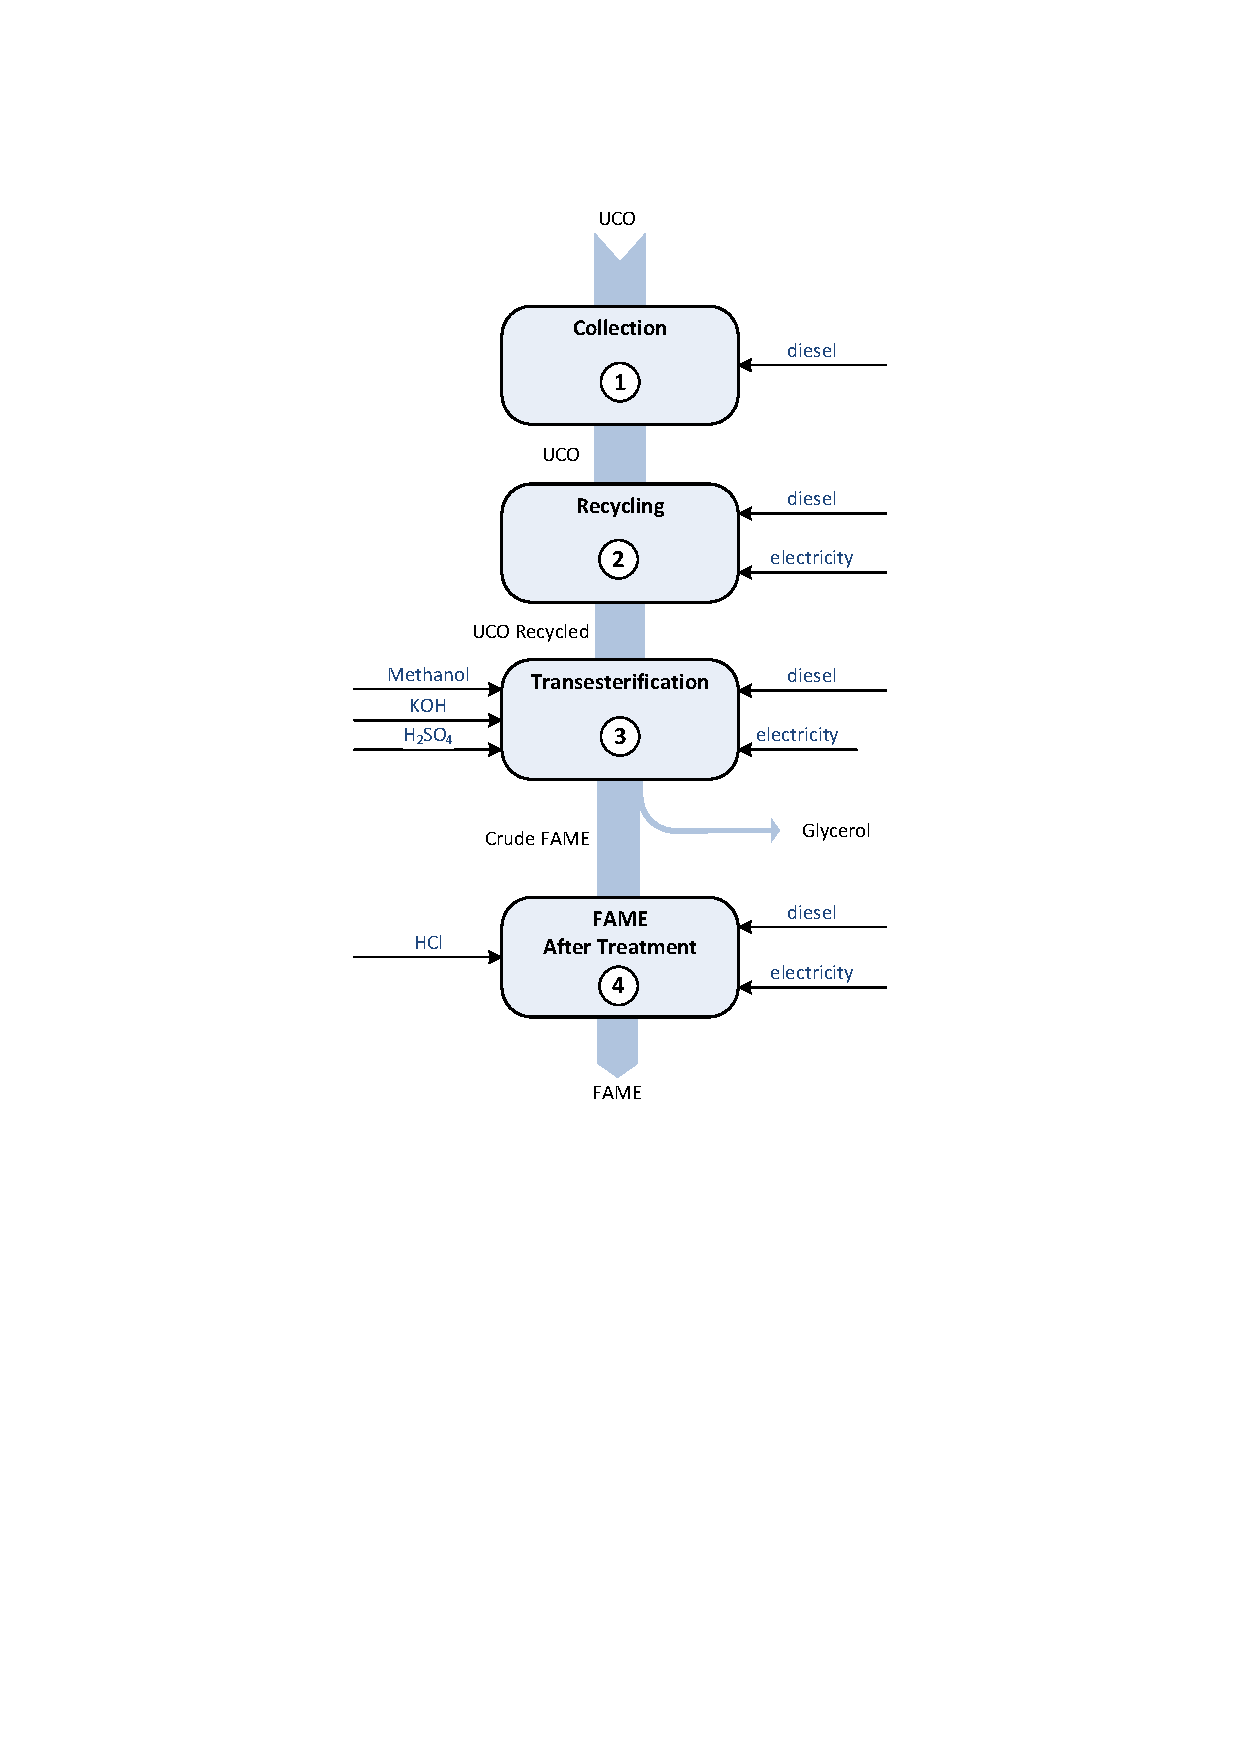
\includegraphics[width=0.5\textwidth]{Figure1}
\caption[Flow diagram of a biodiesel plant producing with Used Cooking Oil]{Flow diagram of a biodiesel plant producing with Used Cooking Oil. Source: CIEMAT \cite{CIEMAT2005}}
\label{fig1}
\end{figure}

The inputs and outputs of the transesterification phase can be seen in \cref{table1} together with flow diagram of \cref{fig1}. These data have been obtained from a LCA carried out by CIEMAT \cite{CIEMAT2005}, based on a supply chain established in the north of Spain and with data of two real biodiesel production plants using this resource. It is important to note that in this case for the production of steam, diesel fuel is considered instead of natural gas.

\begin{table}[htbp]
\centering \small
\caption[Consumption data for processes considered in the life cycle analysis for UCO]{Consumption data for processes considered in the life cycle analysis for UCO. Source: CIEMAT \cite{CIEMAT2005}}
\begin{tabularx}{0.8\textwidth}{lXXXX}
\toprule
\multicolumn{2}{l}{\bf Process} & {\bf I/O}   & {\bf Value} & {\bf Units} \\
\midrule
\multicolumn{5}{l}{\bf Collection} \\
\cmidrule{1-5}
& Diesel & Input & 0.48316 & MJ/kg UCO \\
\cmidrule{1-5}
\multicolumn{5}{l}{\bf Recycling} \\
\cmidrule{1-5}
& Diesel & Input & 0.036 & MJ/kg oil \\
& Electricity & Input & 0.35  & MJ/kg oil \\
\cmidrule{1-5}
\multicolumn{5}{l}{\bf Transesterification} \\
\cmidrule{1-5}
& Recycled oil& Input& 1.03& kg/\kfame \\
& Methanol& Input& 0.155& kg/\kfame \\
& KOH& Input& 0.02770& kg/\kfame \\
& \ce{H2SO4}& Input& 0.017& kg/\kfame \\
& Diesel& Input& 0.455& kWh/\kfame \\
& Electricity & Input& 0.137& kWh/\kfame \\
& FAME & Output & 1.00& kg/\kfame \\
& Glycerol crude& Output& 0.20& kg/\kfame \\
\bottomrule
\end{tabularx}
\label{table1}
\end{table}

\FloatBarrier
%%%%%%%%%%%%%%%%%%%%%%%%%%%%%%%%%%%%%%%%%%

\section{Thermoeconomic Analysis}

The methodology applied in this paper has been introduced in previous works \cite{FontdeMora2012,FontdeMora2013,Torres2012b}. Thermoeconomic Input--Output Analysis, formerly Symbolic Exergoeconomics \cite{Torres2006}, applies the mathematical framework of Input--Output analysis [20] to Exergy Cost Theory \cite{Miller2009}. It provides general relationships between the production demand and the resources cost of an energy system with the efficiency and irreversibilities of each individual process of that system. The distinguishing element in thermoeconomics from conventional energy and exergy analysis is purpose. Matter and energy flows entering and exiting a given system are classified into fuel and product. Fuel (F) refers to the resources that the component uses to achieve its purpose, and product (P) corresponds to the flows related to that purpose \cite{Tsatsaronis1985}.

The system interactions are represented by means of the fuel--product table, see \cref{table2}, which describes how the production processes are related.

\begin{table}[htbp]
  \centering \small
  \caption{Fuel-Product Table}
	  \vskip 2pt
    \begin{tabulary}{\textwidth}{lccCCCCCCc}
    \toprule
          &       & \multirow{2}[6]{1.5cm}{\centering Final Product}  & \multicolumn{5}{c}{Process Resources} &  \\
    \cmidrule(r){4-8}
          &       &    & 1     & $\cdots$     & j     & $\cdots$   & n     & Total \\
		\midrule
External &       &       & \multirow{2}[1]{*}{$E_{01}$} & \multirow{2}[1]{*}{$\cdots$} & \multirow{2}[1]{*}{$E_{0j}$} & \multirow{2}[1]{*}{$\cdots$} & \multirow{2}[1]{*}{$E_{0n}$} & \multirow{2}[1]{*}{$P_0$} \\
     Resources &       &       &       &       &       &       &       &  \\
    \multirow{5}[0]{2cm}{Process Products} & 1     &  $E_{10}$  &  $E_{11}$  & $\cdots$     & $E_{1j}$   &$\cdots$     & $E_{1n}$   & $P_1$ \\
          & $\vdots$     & $\vdots$    & $\vdots$    &    & $\vdots$     &     & $\vdots$    & $\vdots$ \\
          & i     & $E_{i0}$   & $E_{i1}$   & $\cdots$    & $E_{ij}$   & $\cdots$   & $E_{in}$   & $P_i$ \\
          & $\vdots$    & $\vdots$     & $\vdots$     &    & $\vdots$    &    & $\vdots$     & $\vdots$\\
          & n     & $E_{n0}$   & $E_{n1}$   & $\cdots$     & $E_{nj}$   & $\cdots$     & $E_{nn}$   & $P_n$ \\
	  \midrule
    Total &       & $F_0$    & $F_1$    & $\cdots$     & $F_j$    & $\cdots$     & $F_n$    &  \\
    \bottomrule
    \end{tabulary}%
  \label{table2}%
\end{table}%

Let us consider a system formed by, say $n$ processes, and the environment named as process number 0. Let $P_i$ denote the  exergy of the process $i$ production, which is used in part to meet the intermediate requirement as input resources of other processes and in part to meet the final demand of the system. If $E_{ij}$ denotes the exergy of process $i$ uses as resource for process $j$, and $E_{i0}$ denotes the final demand produced in process $i$, the following expression is formed:
\begin{equation}
\label{eq:F}
P_i=E_{i0}+\sum_{j}^{n}E_{ij}, \quad i=1,\ldots,n
\end{equation}
Note that, in this model, the production of the environment $P_0$ is the total exergy of the external resources. On the other hand, the input resources of each process $i$, say $F_i$, is in
part coming from external resources, say $E_{0i}$ and in part from the
production of other processes, then we have the condition:
\begin{equation}
\label{eq:P}
F_i=E_{0i}+\sum_{j}^{n}E_{ji}, \quad i=1,\ldots,n
\end{equation}
\noindent where $F_0$ is the total system demand.

Second Law states that the difference between fuel and product is a positive 
value and equal to the irreversibility (I), accounting for the losses 
appearing in the process: $F_i - P_i = I_i \geq 0$. Furthermore, the unit 
exergy consumption is defined as the ratio between fuel and product: 
$k_i={F_i}/{P_i} \geq 1$

The exergy cost of the products of a system refers to the exergy of the resources consumed to obtain such products. Therefore the exergy cost of the production of a process, denoted as $C_{P,i}$,  is the sum of the cost of the resources consumed by the process: system internals, i.e. products of other processes $C_{ji}$, and the cumulative exergy of the external resources $C_{0,i}$.

\begin{equation}
 C_{P,i}=C_{0,i}+\sum_{j}C_{ij}
 \label{eq1}
\end{equation}

To calculate the production exergy cost, the assumption that the costs of the products obtained in a process are proportional to its exergy is made, see \cite{Lozano1993}:

\begin{equation}
\frac{C_{ij}}{C_{P,i}}=\frac{E_{ij}}{P_i}=y_{ij}
\label{eq2}
\end{equation}

\noindent where $y_{ij}$ is the distribution exergy ratio, which means the portion of production of process $i$ uses as resources of process $j$.

Combining \cref{eq1,eq2} the exergy cost can be calculated by solving the following set of linear equations:

\begin{equation}
C_{P,i}=C_{0i}+\sum_{j=1}^{n}{y_{ji}C_{P,j}} \qquad i=1,..n
\end{equation}

\noindent which could be written in matrix form as:
\begin{equation}
\vm{C}_P = \vm{C}_e + \tmbr{FP} \vm{C}_P
\end{equation}

\noindent where \mbr{FP} is a $(n \times n)$ matrix, whose entries are the distribution exergy ratios, and $\vm{C}_e$ is a $(n \times 1)$ vector, whose entries are the cumulative exergy of the external resources uses in each process.

Therefore, the production cost could be obtained as:

\begin{equation}
 \vm{C}_P =\tmopcr{P} \, \vm{C}_e \qquad \text{where} \qquad \mopcr{P} \equiv \left(\vm{U}-\mbr{FP}\right)^{-1}
 \label{eq4}
\end{equation}
where \mopcr{P} is called production cost matrix, and its elements $\pi_{ij}^{\ast}$ are the global distribution ratios, whose represent the amount of external resources (measured in exergy) of process $i$ required to obtain one exergy unit of the product of the process $j$.
%%%%%%%%%%%%%%%%%%%%%%%%%%%%%%%%%%%%%%%%%%%%%%%%%%
\begin{sidewaystable}[htbp]
  \centering \small
  \caption{Exergy and cost of flows of the UCO biodiesel pathway}
    \begin{tabularx}{0.9\textwidth}{lcccYYYYY}
    \toprule
          &      &   &    &       & \multicolumn{2}{c}{\bf Exergy} & \multicolumn{2}{c}{\bf Cost} \\
    \cmidrule(r){6-7} \cmidrule(r){8-9}
    {\bf Material} & {\bf Process} & {\bf I/O} & {\bf Unit} (u) & u/\kfame & MJ/u  & MJ/\kfame & MJ/u  & MJ/\kfame \\
    \midrule
    Diesel         & 1  & Input  & MJ    & 0.6459 & 1.0000  & 0.6459  & 1.1773  & 0.7604 \\
    UCO            & 1  & Output & kg    & 1.3368 & 39.5994 & 52.9364 &  -      & - \\
    Diesel         & 2  & Input  & MJ    & 0.0371 & 1.0000  & 0.0371  & 1.1773  & 0.0437 \\
    Electricity    & 2  & Input  & MJ    & 0.4679 & 1.0000  & 0.4679  & 2.8690  & 1.3423 \\
    UCO recycled   & 2  & Output & kg    & 1.0300 & 39.5994 & 40.7873 &  -      & - \\
    Methanol       & 3  & Input  & kg    & 0.1550 & 23.1540 & 3.5889  & 30.3074 & 4.6977 \\
    KOH            & 3  & Input  & kg    & 0.0277 & 0.8229  & 0.0228  & 13.3852 & 0.3708 \\
    \ce{H2SO4}     & 3  & Input  & kg    & 0.0170 & 1.6417  & 0.0279  & 2.6295  & 0.0447 \\
    Diesel         & 3  & Input  & MJ    & 1.5651 & 1.0000  & 1.5651  & 1.1773  & 1.8426 \\
    Electricity    & 3  & Input  & MJ    & 0.4713 & 1.0000  & 0.4713  & 2.8690  & 1.3522 \\
    Crude FAME     & 3  & Output & kg    & 1.0100 & 39.8548 & 40.2533 &  -      & - \\
    Crude Glycerol & 3  & Output & kg    & 0.2000 & 23.6779 & 4.7356  &  -      & - \\
    HCl            & 4  & Input  & kg    & 0.0406 & 1.3409  & 0.0544  & 5.2484  & 0.2131 \\
    Diesel         & 4  & Input  & MJ    & 0.0749 & 1       & 0.0749  & 1.1773  & 0.0882 \\
    Electricity    & 4  & Input  & MJ    & 0.0187 & 1.0000  & 0.0187  & 2.869   & 0.0535 \\
    FAME           & 4  & Output & kg    & 1      & 39.8376 & 39.8376 &  -      & - \\
    \bottomrule
    \end{tabularx}%
  \label{table3}%
\end{sidewaystable}%
%%%%%%%%%%%%%%%%%%%%%%%%%%%%%%%%%%%%%%%%%%%%%%%%%%

\Cref{table3} shows the exergy of flows and cumulative exergy of external resources of the UCO biodiesel pathway. From this information the F--P table of the UCO pathway model is built, see \cref{table4}.

\begin{table}[H]
\centering 
\caption[F--P Tables UCO biodiesel]{F--P Tables UCO biodiesel (MJ/kg FAME)}
\begin{tabularx}{0.9\textwidth}{ZZZZZZZ}
\toprule
 & $F_0$  & $F_1$ & $F_2$ & $F_3$ & $F_4$ & Total \\
\midrule
% Table generated by Excel2LaTeX from sheet 'Cost UCO'
$P_0$ &       & 53.58 & 0.51  & 5.68  & 0.15  & 59.91 \\
\cmidrule{1-7}
$P_1$ & 0.00  & 0.00  & 52.94 & 0.00  & 0.00  & 52.94 \\
$P_2$ & 0.00  & 0.00  & 0.00  & 40.79 & 0.00  & 40.79 \\
$P_3$ & 4.74  & 0.00  & 0.00  & 0.00  & 40.25 & 44.99 \\
$P_4$ & 39.84 & 0.00  & 0.00  & 0.00  & 0.00  & 39.84 \\
\midrule
Total & 44.58 & 53.58 & 53.44 & 46.46 & 40.40 &  \\
\bottomrule
\end{tabularx}%
\label{table4}%
\end{table}%

The local and global distribution matrices, are obtained from \cref{table4} using \cref{eq2,eq4}:
\[
\mbr{FP} = \begin{bmatrix}
0.0000 & 1.0000 & 0.0000 & 0.0000 \bigstrut[t]\\
0.0000 & 0.0000 & 1.0000 & 0.0000 \\
0.0000 & 0.0000 & 0.0000 & 0.8947 \\
0.0000 & 0.0000 & 0.0000 & 0.0000 \bigstrut[b]\\
\end{bmatrix}
\qquad
\mopcr{P} = \begin{bmatrix}
1.0000 & 1.0000 & 1.0000 & 0.8947 \bigstrut[t]\\
0.0000 & 1.0000 & 1.0000 & 0.8947 \\
0.0000 & 0.0000 & 1.0000 & 0.8947 \\
0.0000 & 0.0000 & 0.0000 & 1.0000 \bigstrut[b]\\
\end{bmatrix}
\]




 
The production exergy cost can be decomposed \cite{Torres2012b}, considering the different types of resources required. The resources cost vector can be separated into two terms:

\begin{equation}
\label{ce}
\vms{C}{e}=\vms[rs]{C}{e}+\vms[nrs]{C}{e} 
\end{equation}

The first term represents the cumulative exergy of the renewable resources and the latter the non-renewable or fossil resources. Therefore, the exergoecologic cost can be broken down into the renewable and fossil parts: $\vms{C}{P}=\vms[rs]{C}{P}+\vms[nrs]{C}{P}$, where:

\begin{equation}
\label{cpnrs}
\begin{split}
 \vms[rs]{C}{P} &\equiv \tmopcr{P} \vms[rs]{C}{e} \\
 \vms[nrs]{C}{P} &\equiv \tmopcr{P} \vms[nrs]{C}{e}
\end{split}
\end{equation}

This distinction depending on the origin of the resources allows calculating the sustainability indicator. Font de Mora et al. \cite{FontdeMora2012} defined the concept of ExROI and renewability. ExROI measures the amount of product obtained with one unit of non-renewable resources: 

\begin{equation}
\label{exroi}
\textrm{ExROI}=\frac{P}{\ems[nrs]{C}{P}}
\end{equation}

A production process is sustainable if ExROI $>1$. The higher the ExROI value, the more sustainable a production process will be.

Font de Mora et al. \cite{FontdeMora2013}, introduced the concept of renewability ratio, defined as:

\begin{equation}
\label{rho}
\rho=\frac{\ems[rs]{C}{P}}{\ems{C}{P}} \quad 0 \leq \rho \leq 1
\end{equation}
\noindent the portion of renewable resources per total resources used, or the weight of the renewable exergy cost with respect to the total cost.

The results of the cost analysis, obtained by applying \cref{cpnrs},  are shown in \cref{table5}. In this case, the primary UCO stream is considered as a renewable resource and its cost is equal to its exergy. From these values it is possible to compute the ExROI and renewability factor, which are 4.10 and 0.83, respectively. This means that from each unit of non-renewable sources, i.e. fossil fuels, it is possible to obtain 4.10 units of energy and that the percentage of renewable energy contained in the fuel is about 83\%. These values can be increased if the conventional methanol of fossil origin is substituted by a bioproduct, either bioethanol or methanol from biomass.

\begin{table}[htbp]
  \centering
  \caption[Cost analysis for UCO biodisel]{Cost analysis for UCO biodisel (MJ/kg FAME)}
    \begin{tabularx}{0.8\textwidth}{clZZZZZ}
    \toprule
        &                       & $\ems[nrs]{C}{e}$  & $C_P$  & $\ems[rs]{C}{P}$  & $\ems[nrs]{C}{P}$ & $\rho$ \\
    Nr  & Process               & MJ/Kg  & MJ/kg  & MJ/Kg & MJ/kg & \% \\
    \midrule
    1   & Collection            & 0.76   & 53.697 & 52.936 &  0.760 & 98.58 \\
    2   & Refining              & 1.39   & 55.083 & 52.936 &  2.146 & 96.10 \\
    3   & Esterification        & 8.31   & 63.391 & 52.936 & 10.454 & 83.51 \\
    4   & FAME after treatment  & 0.35   & 57.073 & 47.364 &  9.709 & 82.99 \\
    \bottomrule
    \end{tabularx}%
  \label{table5}%
\end{table}%

The values obtained for the UCO biodiesel can be compared to the ones obtained for biodiesels from vegetable oils in \cref{fig3}.  The values for vegetable oils were calculated in \cite{FontdeMoraThesis2013}. As it can be seen, biodiesel production from UCO has the highest ExROI value and the second highest renewability factor, only exceeded by palm oil based biodiesel. The high renewability of palm oil is due to the use of biomass resources to cover part of the energy needs in the cycle. In addition, UCO biodiesel has the lowest non-renewable exergy cost, which means that overall, it consumes less non-renewable resources, i.e. mainly fossil fuels, than its counterparts. The left graphic, in \cref{fig3}, shows also the renewable and non-renewable exergy cost per produced unit of the diferent biodiesels analyzed in the paper. This analysis could be extended to cover also non-edible vegetable oils, for example castor and jatropha oils, and their blends with UCO \cite{Kannan2013}.

\begin{figure}[htbp]
\centering
\subfigure[Renewability ratio]{
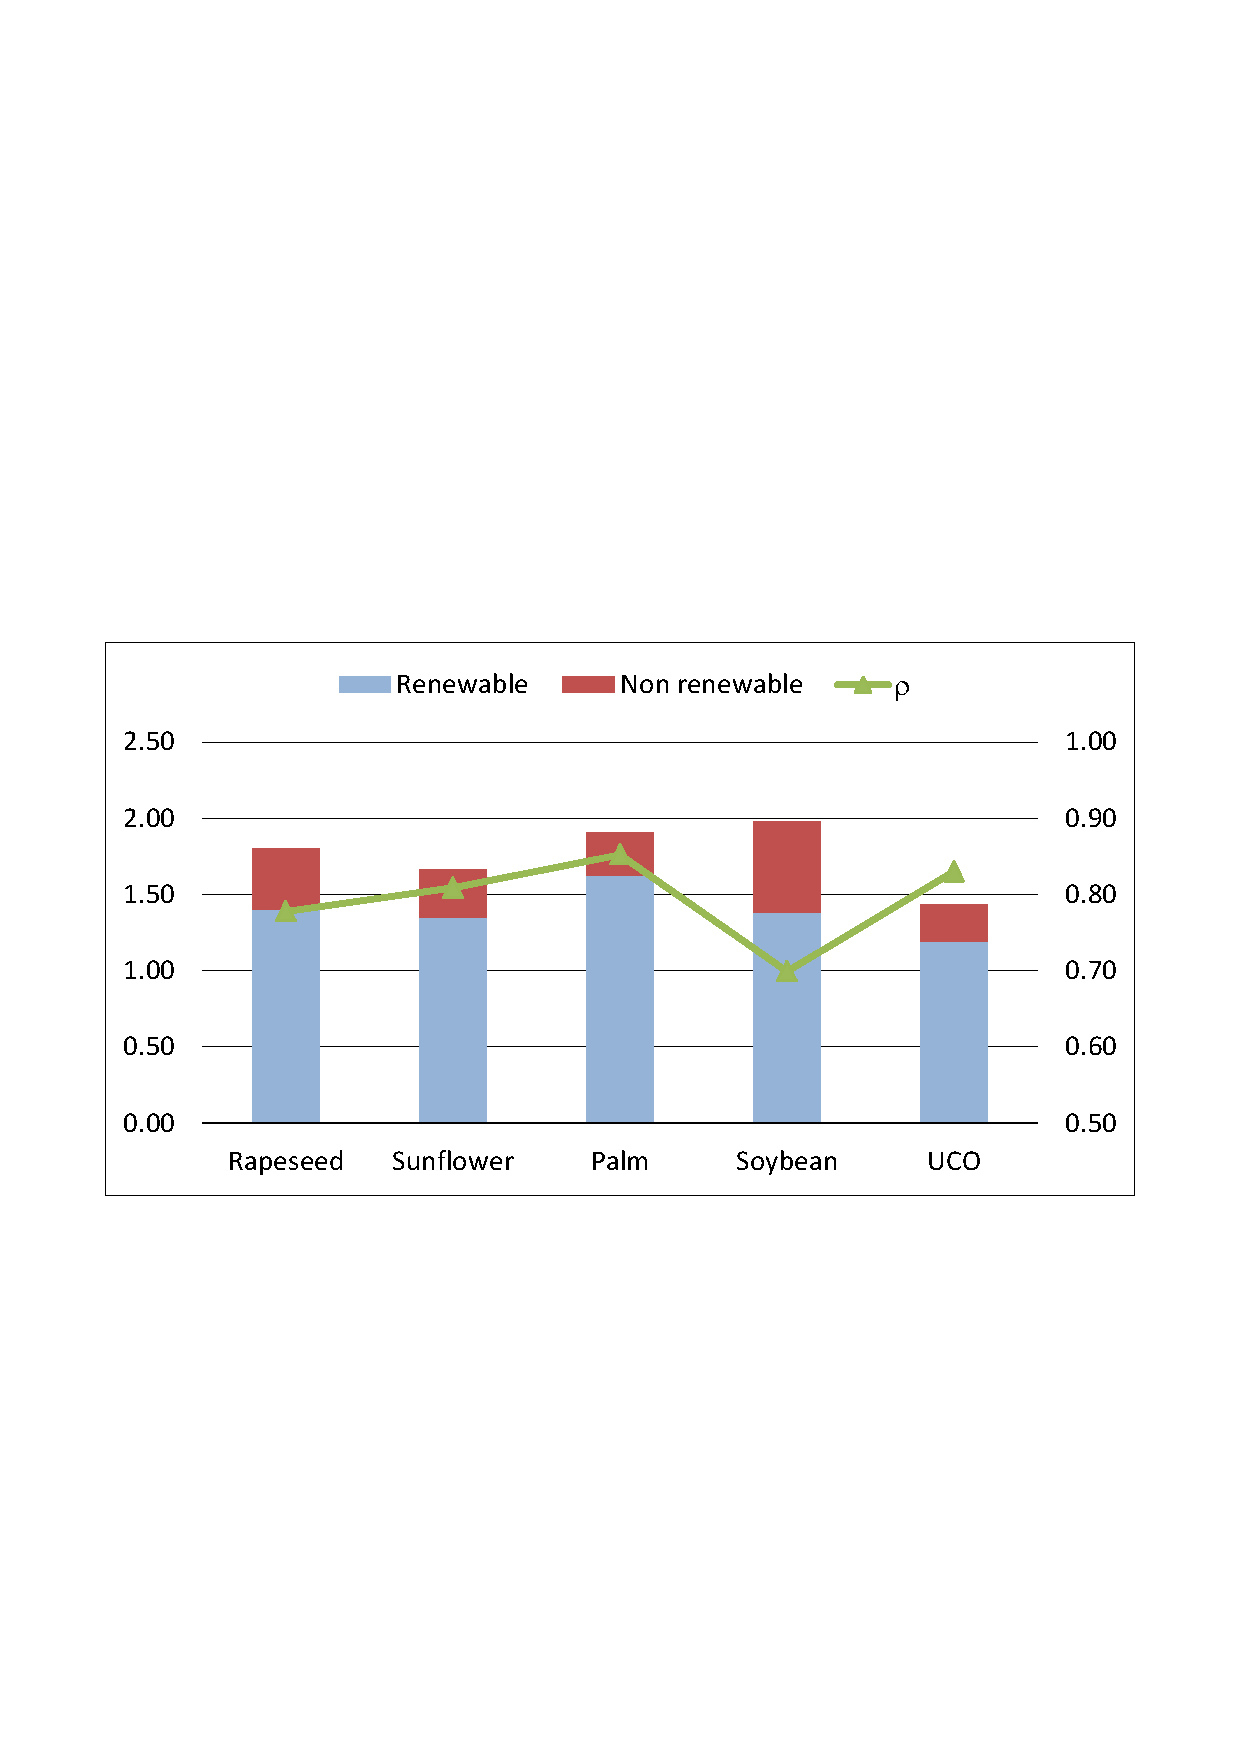
\includegraphics[width=0.48\textwidth]{Figure3a}}
\hfill
\subfigure[ExROI]{
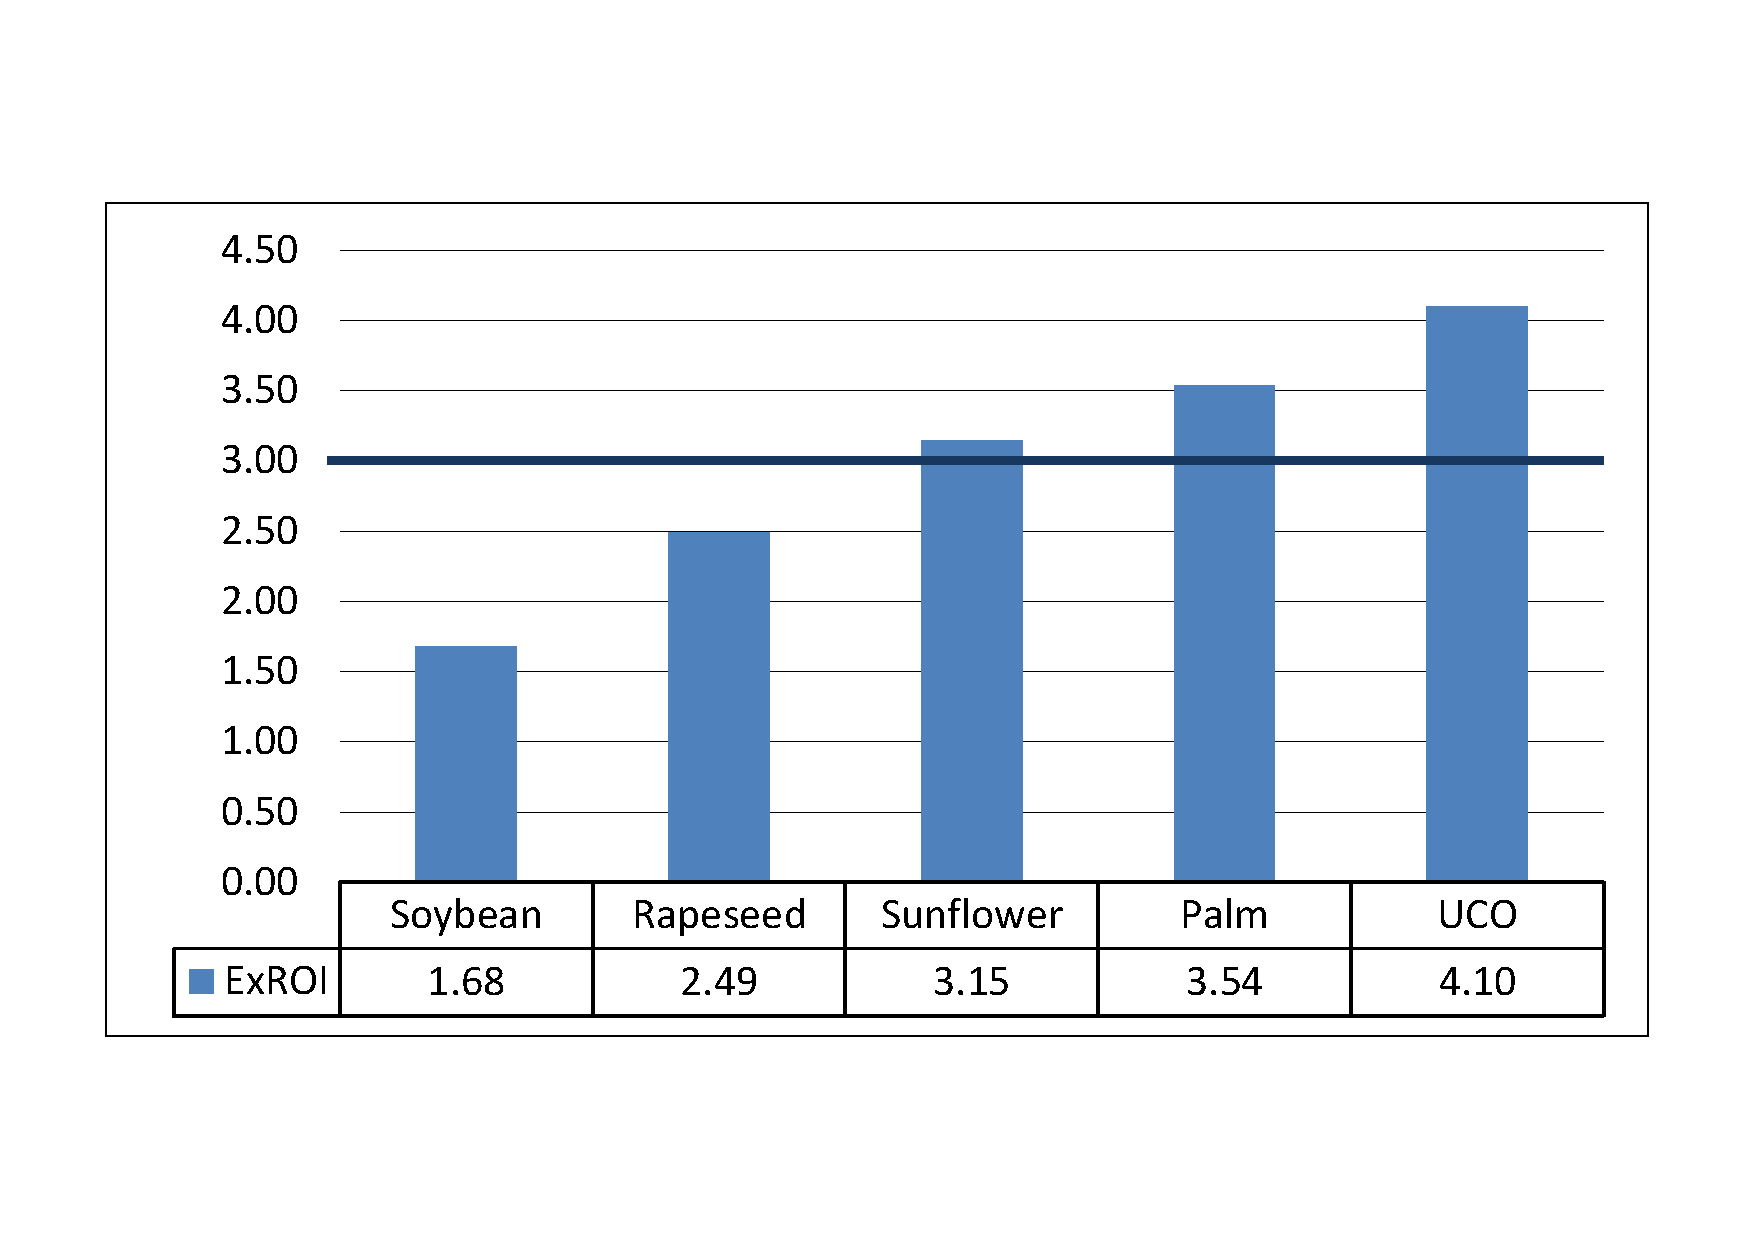
\includegraphics[width=0.48\textwidth]{Figure3b}}
\caption{Comparison of ExROI and Renewability factors of different biodiesel life cycles}
\label{fig3}
\end{figure}

\FloatBarrier
%%%%%%%%%%%%%%%%%%%%%%%%%%%%%%%%%%%%%%%%%%

\section{Analysis of Potential Improvements}

As shown in the previous section, the exergy cost of biodiesel depends on the exergy cost values of the external resources. Therefore, depending on the boundary limits defined by the LCA and from the data provided by LCA databases, whose values may be based on general hypothesis and conversion factors, the results may vary considerably. In order to understand the effect that variations in the consumption of external resources that may have in the production cost values a sensitivity analysis must be performed.

According to \cref{eq4} the cost of the external resources does not depend on the production matrix, thus the effect in the exergy cost due to the variation in the external cost could be calculated as:

\begin{equation}
 \Delta \vm{C}_P =\tmopcr{P} \, \Delta\vm{C}_e
 \label{eq9}
\end{equation}

Introducing the elasticity coefficient $\%\Delta x = \Delta x / x$, \cref{eq9} could be rewritten as:
\begin{equation}
\%\Delta C_{P,i}=\sum\limits_{j=1}^{n}{\frac{C_{0,j}}{C_{P,i}}\pi_{ji}^{\ast}}\,\%\Delta C_{0,j}
\label{eq10}
\end{equation}

This expression is also valid to compute the variation of renewable and non-renewable costs, and
\cref{eq10} could be written in terms of non-renewable costs, as:

\begin{equation}
\label{eq11}
\%\Delta \vms[nrs]{C}{P}= \elm \% \Delta \vms[nrs]{C}{e}
\end{equation}
\noindent where \elm~is called elasticity matrix, whose elements are defined as $a_{ij}=C_{0,j}\pi_{ji}^*/C_{P,i}$. 

\Cref{eq11} could be used to analyse the potential improvements, in terms of sustainability, of replacing non-renewable resources by alternative renewable resources. In case of the life cycle of UCO, its elasticity matrix is:

\[
\elm=\begin{bmatrix} 
1.0000 & 0.0000 & 0.0000 & 0.0000 \bigstrut[t]\\
0.3543 & 0.6457 & 0.0000 & 0.0000 \\
0.0727 & 0.1326 & 0.7974 & 0.0000 \\
0.0702 & 0.1277 & 0.7656 & 0.0365 \bigstrut[b]\\
\end{bmatrix}
\]

From the elasticity matrix, in combination with the information of external resources consumption provided in \cref{table3}, it is possible to obtain the relative impact of the cost of each external resource in the production cost of biodiesel (FAME), which is shown in \cref{table6}. Note, that the sum of each row in the elasticity matrix must be equal to 1.

\begin{table}[htbp]
  \centering
  \caption{Relative impact of external resources on the production cost of FAME from UCO}
    \begin{tabularx}{0.8\textwidth}{lXXXX}
    \toprule
    Flow  & Collection & Recycling & Esterification & FAME \\
    \midrule
    Diesel & 1.0000 & 0.3746 & 0.2532 & 0.2530 \\
    Methanol & 0.0000 & 0.0000 & 0.4433 & 0.4273 \\
    Electricity & 0.0000 & 0.6254 & 0.2594 & 0.2554 \\
    KOH   & 0.0000 & 0.0000 & 0.0350 & 0.0337 \\
    \ce{H2SO4} & 0.0000 & 0.0000 & 0.0042 & 0.0041 \\
    HCl   & 0.0000 & 0.0000 & 0.0000 & 0.0217 \\
    \bottomrule
    \end{tabularx}%
  \label{table6}%
\end{table}%

The non-renewable resource having higher impact in the production cost of FAME is methanol 42.73\%. It means that, if we replace methanol by bio-methanol obtained from wood \cite{Bailey2013,FontdeMoraThesis2013}, the non-renewable production cost of FAME produced from UCO decreases in 42.73\%, and the ExROI value is increased up to 7.07.

By recycling 7\% biodiesel (82\% renewable source) to produce the required electricity in the production of FAME, the production cost is reduced 0.2554 $\times$ 82.8\% $=$ 21.15\%, and the ExROI is increased up to 5.10.

By using part of the produced biodiesel in the collection process, in order to substitute the consumption of diesel, the production cost will be reduced 0.0692 $\times$ 82.8\% $=$ 5.73\%,  and the ExROI will be increased up to 4.28.

Finally, if several measures are combined, like the use of organic methanol and the recirculation of 16\% of the biodiesel (6.3 MJ/kg) to substitute part of the energy needs in the process, the ExROI would be increased to 69 and the renewability to 98.7\%.

%%%%%%%%%%%%%%%%%%%%%%%%%%%%%%%%%%%%%%%%%%

\section{Conclusions}

This paper applies the methodology and concepts introduced in \cite{FontdeMora2012,FontdeMora2013,Torres2012b} to the life cycle production of biodiesel produced from used cooking oils. Used cooking oils have the potential to replace 1.5--1.8\% of the EU-27 diesel consumption with a GHG emission reduction potential of 88\% compared to fossil diesel. Given the importance that this alternative fuel is gaining and the support that is given by the energy and transport policy frameworks worldwide, it is important to assess its life cycle from the thermoeconomic perspective, analyse how the process can be improved and compare the results with other biodiesel types. The results show that biodiesel from used cooking oil is the most sustainable biodiesel from the point of view of the use of non-renewable resources. The ExROI value is higher than 3, which is, according to Hall et al. \cite{Hall2009}, the minimum EROI value that society must attain from its energy exploitation to support continued economic activity and social function. The most important measure to improve the production cycle is substituting the fossil derived methanol by an alcohol of biological origin, which provides an ExROI increase of 75\%.

%=================================================================
% References
%=================================================================
\makeatletter
\renewcommand\@biblabel[1]{#1.}
\makeatother
\bibliography{Turriano}
\bibliographystyle{mdpi}

%%%%%%%%%%%%%%%%%%%%%%%%%%%%%%%%%%%%%%%%%%
\abbreviations{Nomenclature}
\begin{list}{}{
    \renewcommand*{\makelabel}[1]{\hspace{\labelsep}\raggedleft #1}  
    \setlength{\labelwidth}{3em}
    \setlength{\leftmargin}{\labelwidth}
    \setlength{\parsep}{0pt}
    \setlength{\itemsep}{0pt}
    \sloppy}
    \item[c] Unit Exergy Cost (MJ/MJ)
    \item[n] Number of processes
    \item[C] Exergy Cost (MJ/kg FAME) 
    \item[F] Exergy of Fuel (MJ/kg FAME)
    \item[P] Exergy of Product (MJ/kg FAME)
    \item[y] Exergy distibution ratios (MJ/MJ)
    \item[$\rho$] Renewability ratio (\%)
    \item[$\pi^*$] Global distribution ratios (MJ/MJ)
\end{list}

\noindent\emph{Matrix and Vectors}
\begin{list}{}{
\renewcommand*{\makelabel}[1]{\hspace{\labelsep}\raggedleft #1}  
    \setlength{\labelwidth}{3em}
    \setlength{\leftmargin}{\labelwidth}
    \setlength{\parsep}{0pt}
    \setlength{\itemsep}{0pt}
    \sloppy}
    \item[\mbr{FP}] Exergy distribution ratios matrix $(n \times 1)$
    \item[$\vm{C}_e$] Vector of external resources $(n \times 1)$
    \item[\mopcr{P}] Production cost operator matrix $(n \times n)$
    \item[$\vm{U}_n$] Identity Matrix $(n \times n)$
    \item[\elm] Elasticity Matrix $(n \times n)$
\end{list}

\noindent\emph{Subscripts and supersccripts}
\begin{list}{}{
    \renewcommand*{\makelabel}[1]{\hspace{\labelsep}\raggedleft #1}  
    \setlength{\labelwidth}{3em}
    \setlength{\leftmargin}{\labelwidth}
    \setlength{\parsep}{0pt}
    %\setlength{\topsep}{0pt}
    \setlength{\itemsep}{0pt}
    \sloppy}
    \item[0] Environment process
    \item[e] External resources
    \item[F] Fuel
    \item[nrs] Non renewable resources
    \item[P] Product
    \item[rs] Renewable resources
    \item[T] Transpose Matrix
\end{list}

\noindent\emph{Abbreviations}
\begin{list}{}{
	\renewcommand*{\makelabel}[1]{\hspace{\labelsep}\raggedleft #1}
    \setlength{\labelwidth}{6em}
    \setlength{\leftmargin}{\labelwidth}
    \setlength{\parsep}{0pt}
    \setlength{\itemsep}{0pt}
    \sloppy}
    \item[CIEMAT] Centro de Investigaciones Energ\'eticas, Medioambientales y Tecnol\'ogicas
    \item[EC] European Commission
    \item[EROI] Energy Return of Energy Investment
    \item[EU] European Union
    \item[EU-27] European Union comprising 27 member states (excluding Croatia)
    \item[ExROI] Exergy Return of Exergy Investment
    \item[FAME] Fatty Acid Methyl ester (biodiesel)
    \item[FFA] Free Fatty Acid
    \item[GEREGRAS] Spanish association of vegetable oil and fat residues management companies
    \item[HORECA] Sector of the food service industry
    \item[LCA] Life Cycle Analysis
    \item[UCO] Used Cooking Oil
\end{list}

\end{document}